\documentclass[11pt,a4paper]{article}
\usepackage{graphicx}
\usepackage{amssymb}
\DeclareGraphicsExtensions{.pdf,.png,.jpg}

\begin{document}

\title{CS6690: Pattern Recognition Assignment \#2}
\author{Group 3: Akshay \& Suthirth}
\maketitle

\newpage

\section{Bayesian Classifiers}
According to Bayes Theorem, for a dataset x with classes $\omega_i$, \\
Probability of a datapoint belonging to class $\omega_i$ is defined as: \\
\begin{equation}
P(\omega_i | x) = \frac{(P(x|\omega_i)P((\omega_i))}{P(x)}
\end{equation}
\\ 

\begin{itemize}

	\item Here, $P(x|\omega_i)$ is known as the class likelihood. 
\\ To estimate this value, we require the distribution of $\omega_i$.
Based on the central limit theorem, we can assume that this would be Gaussian distribution for large datasets. 

	\item The value $P(\omega_i)$ is the class prior and is calculated using:
		\begin{equation}
		P(\omega_i) = N_i / N  
		\end{equation}
	This term becomes irrelevant if the classes have equal probabilities. 

	\item P(x) is termed as 'evidence' and can be calculated as:
	\begin{equation}
	{P(x) = \sum_i P(x | \omega_i)P(\omega_i)}
	\end{equation}
\end{itemize}

\section{Gaussian Likelihood Distribution}
 
 For multi-dimensional data, the Gaussian Distribution is:   
 \begin{equation}
 P(x;\mu,\Sigma) = \frac{1}{2\pi^{k/2}|\Sigma|^{1/2}} e^{-(x-m)^{T} \Sigma^{-1} (x-m)}
 \end{equation}
 
 where
 \begin{itemize}
 	\item $\mu$ is the mean 
 	\item $\Sigma$ is the covariance matrix
 \end{itemize}
 
 The above parameters are calculated for the following cases:
 \subsection{Bayes Classifier with Covariance same for all classes}
 \subsection{Bayes Classifier with Covariance different for all classes}
 \subsection{Naive Bayes Classifier with C = $\Sigma^2*I$}
 \subsection{Naive Bayes Classifier with C same for all classes}
 \subsection{Naive Bayes Classifier with C different for all classes} 

\section{Bayes Classification}

If $P(\omega_1 | x) > P(\omega_2 | x)$ then x belongs to class $\omega_1$
\\If $P(\omega_1 | x) < P(\omega_2 | x)$ then x belongs to class $\omega_2$\\

Using equation (1), this can be written as:
 \begin{equation}
 {P(x| \omega_1)P(\omega_1) \gtrless P(x | \omega_2)P(\omega_2)}
 \end{equation}

This classification rules minimizes number of misclassifications. 

\section{Experiments}

\subsection{Data}
\begin{figure}[h!]
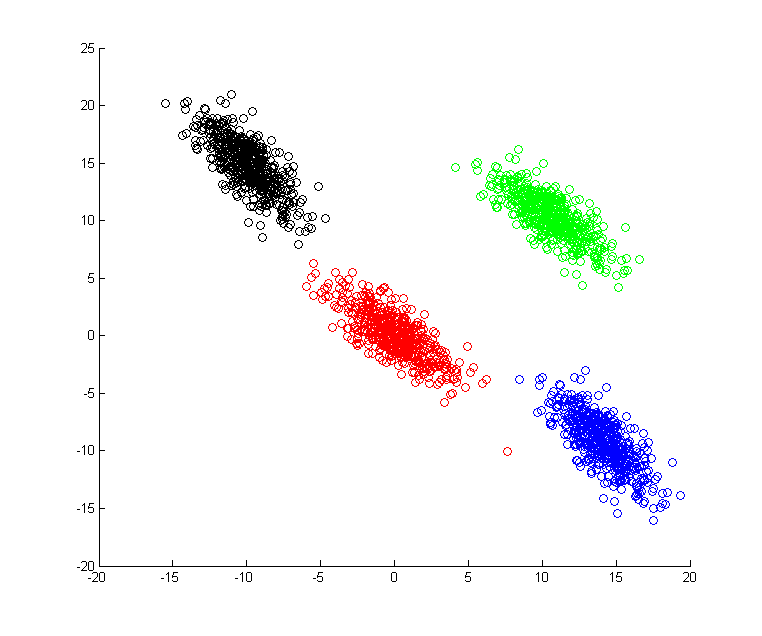
\includegraphics[width=10cm]{ls_group3.png}
\caption{Linearly Separable Data}
\end{figure}

\subsection{Parameters}
\subsection{DET Curves}
\subsection{Decision Boundaries}
\subsection{Confusion Matrices}

\section{Cases}
\subsection{Subsection Heading Here}
Write your subsection text here.

\begin{figure}
    \centering
  %  \includegraphics[width=3.0in]{myfigure}
    \caption{Simulation Results}
    \label{simulationfigure}
\end{figure}

\section{Conclusion}
Write your conclusion here.

\end{document}